\section{Background: Safe Kernel Extensions}
\label{sec:background}
\djw{thinking about this being ``background and motivation'' with this being the first half and 3 being the section half}

%% \subsection{eBPF}
%% eBPF is a Linux kernel subsystem that allows for safe and dynamic kernel extension.
%% Developers write programs that get compiled to eBPF bytecode before being verified by an in-kernel verifier.
%% The verifier ensures certain safety properties about the programs such as termination and memory safety.
%% The execution of eBPF programs follows an event based mechanism, where control flow will transfer to the extension when certain events happen in the system.
%% eBPF programs also have access to a set of helper functions inside the kernel, which allow them to interact with kernel state.
%% Recent work has argued that the safety guarantees of the eBPF verifier are not as strong as claimed, especially in respect to the helper function interface \cite{untenableVerification}.

%% %\begin{itemize}
%% %    \item extension program model
%% %    \item verification
%% %    \item helpers
%% %    \item eBPF problems, echo the HotOS paper
%% %\end{itemize}

%% \subsection{Rust}

%% \juowen{TODO: maybe add some content related to Rust's syntactic sugar}
%% \begin{itemize}
%%     \item language-based safety
%%     \item expressiveness
%% \end{itemize}
%% \hubertus{you have to describe what "safe Rust" vs. "regular Rust" is, you should also highlight the popularity of Rust "https://medium.com/@codilime/the-future-of-rust-characteristics-popularity-and-challenges-7de4db5ebd67"}
%% % \subsection{Rust v.s. eBPF}
%% %
%% % \begin{itemize}
%% %     \item Probably has a better place
%% %     \item Sets and examples we discussed
%% %         \begin{itemize}
%% %             \item Rust and eBPF: Small, simple programs
%% %             \item eBPF but not Rust: certain code is unsafe in Rust but safe in
%% %                 eBPF, e.g. reinterpreting bytes in a packet into another struct
%% %             \item Rust but not eBPF: Expressiveness argument
%% %         \end{itemize}
%% % \end{itemize}


%% \subsection{Threat Model for Safe Kernel Extensions}
%% Part of the success of eBPF in the industry stems from its claim of
%% safety, achieved by the in-kernel verifier.  For example, as opposed
%% to Linux kernel modules (written in C), safety in eBPF lowers the
%% barrier to entry and trust required for system administrators to
%% install an extension into a production system.  However, there are
%% ongoing debates in industry~\cite{unprivileged-ebpf} and
%% academia~\cite{untenableVerification} about the quality of eBPF's safety
%% guarantees and in what circumstances they can be relied on.  Here we
%% specify the threat model and expectations for safety of kernel
%% extensions for the scope of this paper.

%% We assume that extensions are installed by a system administrator with
%% root privileges on the system.  Extensions are written by well-meaning
%% but imperfect developers and thus may contain programming mistakes.
%% We assume that the extension is not actively malicious.  So called
%% ``guarantees'' of safety therefore consist of the best-effort catching
%% of common mistakes.  While some in the community may be interested in
%% exploring stronger notions of
%% safety~\cite{unprivileged-ebpf,jia2023}, we note that this
%% definition of safety is consistent with the current eBPF ecosystem,
%% where actively malicious extension writers can crash or hang the
%% system~\cite{untenableVerification,ebpf-stackoverflow,ebpf-termination} (e.g.,
%% via helper functions), but the verifier prevents obvious mistakes (e.g.,
%% dereferencing a NULL pointer).




Kernel extensions allow code to be added to the kernel dynamically at
runtime for usecases ranging from observability and monitoring to
customization and acceleration.  Whereas safety of extensions was once
only a concern of the research community (e.g., SPIN~\cite{spin},
VINO~\cite{vino}, etc.), the shortening space between development,
debugging and deployment in today's industry landscape has created a
need for extending systems in production, where any system instability
caused by extensions is difficult to tolerate.

As a result, the past decade has seen the re-emergence of safety
concerns for kernel extensions, embodied in Linux by the eBPF
ecosystem.  Unlike the Linux kernel module framework, where modules
are written in C and programmer errors (e.g., errant pointer
dereferences, integer overflows) will crash the kernel, the eBPF
framework attempts to limit the damage from extension programmer error
by compiling extensions written in a high-level language like C or
Rust to a bytecode representation that is checked at extension load
time by an in-kernel verifier.  This workflow is shown in
Figure~\ref{fig:gap}.

%% \begin{figure}
%%     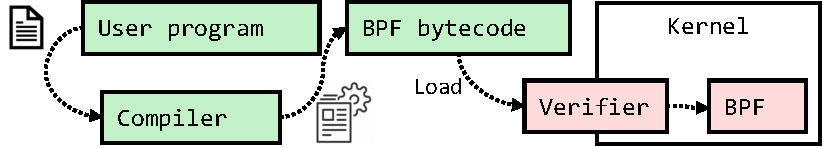
\includegraphics[width=1.0\linewidth]{figs/bpf_intro.pdf}
%%     \centering
%%     \vspace{-10pt}
%%     \caption{Overview of eBPF}
%%     \label{fig:ebpf}
%%     \vspace{-10pt}
%% \end{figure}

The safety properties checked by the eBPF verifier are generally
related to avoiding kernel crashes or hangs.  In eBPF, the verifier
uses a form of symbolic execution on the bytecode to examine all
possible executions to ensure safety.  It also performs limited
checks on the extension's
interactions with the kernel through {\em
  helper functions}.
We characterize these verifier
checks as ensuring the following conceptual properties of the
extension:
\begin{itemize}
\item {\bf Memory Safety:} Extensions can only access memory that is
  provided to them through explicit context arguments or kernel
  interfaces, (e.g., helper functions).  This prevents kernel crashes
  through NULL pointer dereference or corruption of kernel data
  structures.
\item {\bf Type Safety:} When accessing data in memory, the extension must use
  the correct type of the data. This helps avoid misinterpretation of the data
  or memory corruptions.
% When invoking kernel interfaces, the
%   extension must supply arguments of the appropriate type.  This helps
%   avoid kernel crashes in helper functions.
\item {\bf Resource Safety:} When gaining access to kernel objects
  (e.g., lock, allocated memory, etc.) through helper function,
  extensions must subsequently invoke the appropriate release
  interface on the object before completion.  This prevents memory
  leaks or deadlocks that can hang or crash the kernel.
\item {\bf Runtime Safety:} Extensions must terminate. This prevents
  infinite loops that hang the kernel indefinitely.
\item {\bf Undefined Behavior Elimination:} Extensions must never
  exhibit undefined behavior, including integer errors (e.g.,
  overflow, divide by zero, etc.). This prevents runtime kernel
  crashes.
\item {\bf Stack safety:} A unique safety requirement for kernel exntensions.
  Extension must not overflow the limited kernel stack.
  Failing to do so risks kernel crashes or kernel memory corruption.
\end{itemize}

This notion of safety in eBPF lowers the barrier to entry and trust
required for system administrators to install an extension into a
production system.  However, there are ongoing debates in
industry~\cite{reconsider-unpriv-ebpf-lwn,seccomp-ebpf-lwn,ebpf-sec-lwn} and
academia~\cite{untenableVerification} about the quality of eBPF's
safety guarantees and in what circumstances they can be relied on.
Here we specify the safety model and expectations for safety of kernel
extensions for the scope of this paper.

\paragraph{Safety model:} We assume that extensions are installed by a system administrator with
root privileges on the system.  Extensions are written by well-meaning
but imperfect developers and thus may contain programming mistakes.
We assume that the extension is not actively malicious.  So called
``guarantees'' of safety therefore consist of the best-effort catching
of common mistakes.  While some in the community may be interested in
exploring stronger notions of safety~\cite{reconsider-unpriv-ebpf-lwn,seccomp-ebpf-lwn,ebpf-sec-lwn,jia2023},
we note that this definition of safety is consistent with the current
eBPF ecosystem, where actively malicious extension writers can crash
or hang the
system~\cite{untenableVerification,ebpf-stackoverflow,ebpf-termination}
(e.g., via helper functions), but the verifier prevents obvious
mistakes (e.g., dereferencing a NULL pointer).
